\subsection{Genus}
\index{genus|(}%
%label{sec:genus}%
Zanim przejdziemy do zdefiniowania macierzy Seiferta, potrzebować będziemy krótkiego skoku w bok -- zrozumieć bardzo geometryczny niezmiennik węzłów, genus.

Zaczniemy od starego twierdzenia, które klasyfikuje powierzchnie domknięte.

\begin{proposition}
    Każda powierzchnia domknięta jest członkiem jednej z dwóch nieskończonych rodzin:
    \begin{enumerate}[leftmargin=*]
        \itemsep0em
        \item sumą spójną $g \ge 0$ torusów,
        \item sumą spójną $k \ge 1$ rzeczywistych płaszczyzn rzutowych.
    \end{enumerate}
\end{proposition}

Elementy pierwszej rodziny są orientowalne.
Sferę traktujemy dla wygody jako sumę spójną $g = 0$ torusów.
Wtedy sumę spójną $g$ torusów możemy wyobrazić sobie jako sferę, do której doklejono $g$ uchwytów.

\begin{definition}[genus powierzchni]
    Ilość torusów nazywamy genusem powierzchni i oznaczamy literą $\genus$.
\end{definition}

Podobna charakteryzacja istnieje dla powierzchni z~brzegiem.
Każdy taki obiekt jest homeomorficzny z~sumą spójną $g$ torusów, w~których wydrążono pewną liczbę otworów: tyle, ile składowych spójności ma brzeg powierzchni.
W~przypadku powierzchni Seiferta mamy do czynienia z jednym otworem.

Dla wygody przypomnijmy jeszcze definicję klasycznego niezmiennika powierzchni:

\begin{definition}[charakterystyka Eulera]
\index{charakterystyka Eulera}%
    Niech $M$ będzie domkniętą powierzchnią orientowalną.
    Po striangulowaniu, składa się z $k_0$ wierzchołków, $k_1$ krawędzi oraz $k_2$ ścian.
    Wielkość
    \begin{equation}
        \chi = k_0 - k_1 + k_2
    \end{equation}
    jest niezmiennikiem powierzchni, zwanym charakterystyką Eulera.
\end{definition}

Definicja ta nie jest wygodna podczas ręcznych obliczeń.
Mamy za to:

\begin{proposition}
    Charakterystykę Eulera powierzchni jednoznacznie wyznaczają cztery reguły:
    \begin{itemize}
        \item jeśli $M$ jest dyskiem, to $\chi(M) = 1$,
        \item jeśli $M_1, M_2$ są powierzchniami, to $\chi(M_1 \sqcup M_2) = \chi(M_1) + \chi(M_2)$,
        \item jeśli powierzchnia $M_2$ powstaje z $M_1$ przez dołączenie paska, to $\chi(M_2) = \chi(M_1) - 1$,
        \item jeśli powierzchnia $M_2$ powstaje z $M_1$ przez dołączenie dysku do całej składowej spójności brzegu, to $\chi(M_2) = \chi(M_1) + 1$.
    \end{itemize}
\end{proposition}

Genus oraz charakterystyka Eulera są ze sobą związane:

\begin{proposition}
    Niech $M$ będzie powierzchnią o genusie $\genus$ i $\mu$ składowych spójności brzegu.
    Wtedy
    \begin{equation}
        \chi = 2 - \mu - 2\genus.
    \end{equation}
\end{proposition}

Nas interesują głównie powierzchnie Seiferta węzłów:
\index{powierzchnia Seiferta}

\begin{proposition}
    \label{prp:seifert_euler_characteristics}
    Niech $K$ będzie węzłem z~diagramem $D$.
    Wtedy $\chi(M_D) = d - b$, gdzie $b$ jest liczbą skrzyżowań $D$, zaś $d$ jest liczbą okręgów Seiferta.
\end{proposition}

Można przeczytać o tym w \cite[s. 82]{murasugi96}.

\begin{proof}
    W~dowodzie faktu \ref{prp:seifert_exists} widzieliśmy, że liczba skrzyżowań $b$ jest jednocześnie liczbą pasków doklejonych do dysków.
    Bezpośredni rachunek pokazuje, że wtedy $k_0 = 4b$, $k_1 = 6b$ oraz $k_2 = b+d$.
    Wynika stąd, że $\chi = 4b - 6b + b + d = d - b$.
\end{proof}

Reszta tej podsekcji nie jest wymagana do zrozumienia macierzy Seiferta, przyjrzymy się genusowi jako obiektowi ciekawemu samemu w sobie.

\begin{definition}[3-genus]
    Niech $K$ będzie węzłem.
    Wśród wszystkich powierzchni Seiferta węzła $K$ istnieje co najmniej jedna o minimalnym genusie, jej genus nazywamy 3-genusem węzła $K$ i oznaczamy także przez $\genus$.
\end{definition}

Znalezienie 3-genusu dowolnego węzła sprawia te same trudności, co wyznaczenie jego liczby gordyjskiej.
Dowolna powierzchnia Seiferta zadaje ograniczenie z góry.
Z dołu 3-genus można szacować przy użyciu wielomianu Alexandera:
\index{wielomian!Alexandera}%

\begin{proposition}
    \label{prp:alexander_genus}
    Niech $K$ będzie węzłem.
    Wtedy $\operatorname{span} \alexander_K(t) \le 2\genus(K)$.
\end{proposition}

Fakt ten znalazłem w podręczniku Murasugiego \cite[s. 131]{murasugi96}.

\begin{proof}
    Załóżmy, że $F$ jest powierzchnią Seiferta węzła $K$ o genusie $g$.
    Wtedy macierz Seiferta powstała z $F$ jest stopnia $2g$, więc żaden ze składników jej wyznacznika nie może mieć stopnia (jako wielomian) większego niż $2g$.
\end{proof}

To dolne ograniczenie jest realizowane przez pewną powierzchnię Seiferta dla każdego pierwszego węzła o~co najwyżej 11 skrzyżowaniach poza siedmioma wyjątkami: 11n42, 11n67, 11n97 ($g = 2$), 11n34, 11n45, 11n73 oraz 11n152 ($g = 3$).
% warto byłoby dodać jakiś kod pozwalający sprawdzić, czemu akurat te węzły
Jeżeli nie powoduje to nieporozumień, zamiast 3-genus można pisać po prostu genus.

\begin{proposition}
    Niech $K$ będzie węzłem, zaś $M$ jego macierzą Seiferta.
    Równość $\operatorname{span} \alexander_K(t) = 2\genus(K)$ zachodzi wtedy i tylko wtedy, gdy wyznacznik $\det M \neq 0$ jest niezerowy.
\end{proposition}

Floer zdefiniował w~\cite{floer90} przestrzeń wektorową nazywaną teraz homologią Floera, jest ona wyposażona w~endomorfizm parzystego stopnia, który powstaje z 2-wymiarowej klasy homologii reprezentowanej przez powierzchnię Seiferta.
%~kanoniczną gradację modulo $2$ oraz
\index{homologia!Floera}
Ta homologia rozkłada się na sumę prostą przestrzeni własnych wyróżnionego endomorfizmu, ich charakterystyki Eulera są współczynnikami wielomianu Alexandera.
Pozwala to na dokładniejsze szacowanie genusu węzła, patrz prace Ozsvátha, Szabó \cite{szabo03} i Ghigginiego \cite{ghiggini08}.

Z góry genus ograniczony jest przez kilka klasycznych niezmienników numerycznych.
Zanim to pokażemy, przytoczymy techniczny lemat udowodniony przez Yamadę (\cite{yamada87}):

\begin{proposition}
    \label{prp:seifert_circles_braid}
    Niech $L$ będzie splotem, zaś $\operatorname{s} L$ minimalną liczbą okręgów Seiferta, które dostajemy ze wszystkich możliwych diagramów splotu $L$.
    Wtedy $\operatorname{s} L = \braid L$ jest równe indeksowi warkoczowemu.
\index{indeks warkoczowy}%
\end{proposition}

Powyższe stwierdzenie występuje bez dowodu (bez?) w \cite[s. 17]{kawauchi96}.

\begin{proposition}
    Niech $L$ będzie splotem.
    Wtedy $\crossing L - \braid L - \operatorname{\mu} L + 2 \ge 2 \genus L$.
\end{proposition}

\begin{proof}
    Ustalmy minimalny diagram $D$ dla splotu $L$ i zastosujmy do niego algorytm Seiferta.
    Dostaniemy tak $s$ okręgów Seiferta oraz powierzchnię o genusie $g$.
    Fakt \ref{prp:seifert_euler_characteristics} mówiący, że $\chi = s - c$, można przekształcić do
    \begin{equation}
        g = \frac{c + 2 - s - \mu(K)}{2}.
    \end{equation}
    Z~minimalności diagramu wynika, że $c = \crossing L$.
    Fakt \ref{prp:seifert_circles_braid} mówi, że $s \ge \braid L$.
    Nierówność $g \ge \genus L$ wynika z~definicji genusu.
    Z powyższych rozważań wynika, że
    \begin{equation}
        \crossing L + 2 \ge 2 \genus L + \braid L + \operatorname{\mu} L,
    \end{equation}
    a to jest równoważnie nierówności, której prawdziwości dowodzimy.
\end{proof}

\begin{corollary}
    \label{cor:crossing_genus}
    Niech $K$ będzie węzłem.
    Wtedy $\crossing K \ge 2 \genus K$.
\index{indeks skrzyżowaniowy}
\end{corollary}

Czy w definicji genusu można ograniczyć się do powierzchni Seiferta, które pochodzą od algorytmu Seiferta?
Niestety, poza pewnymi wyjątkami, nie.
Zanim przekonamy się, dlaczego tak jest, zdefiniujmy jeszcze dwa niezmienniki.

\begin{definition}[genus kanoniczny]
\index{genus!kanoniczny}%
    Niech $K$ będzie węzłem.
    Najmniejszy z genusów powierzchni Seiferta węzła $K$, które pochodzą z~algorytmu Seiferta, nazywamy genusem klasycznym i~oznaczamy symbolem $\operatorname{g_c} K$ lub krótko $g_c$.
\end{definition}

Stojmenow \cite{stoimenow08} opisał diagramy węzłów o~kanonicznym genusie równym 2.
Część z~jego wyników przenosi się na genus 3.
Jak sam pisze, sklasyfikowane wcześniej węzły o~genusie (kanonicznym) 1 okazały się być zbyt wąską klasą.

Pod koniec lat pięćdziesiątych Crowell i~Murasugi niezależnie zauważyli, że algorytm Seiferta zastosowany do alternującego diagramu zawsze daje powierzchnię o~minimalnej powierzchni.
Ich kombinatoryczne uzasadnienie było dość zawiłe, elementarny dowód podał Gabai w \cite{gabai86}.

Dubel trójlistnika ma genus równy $1$, ale algorytm Seiferta zastosowany wobec węzła produkuje powierzchnie o genusie co najmniej $3$, jak przewiduje ograniczenie znalezione przez Mortona w \cite[twierdzenie 2]{morton86}:

\begin{proposition}
    Niech $P(v, z)$ będzie wersją wielomianu HOMFLY spełniającą zależność
    \begin{equation}
        \frac 1v P_+ - vP_- = zP_0.
    \end{equation}
    Wtedy $M = \max \deg_z P(v, z) \le 2g_c$.
\end{proposition}

Nierówność Mortona jest równością dla wielu klas węzłów, w tym alternujących (Crowell, Murasugi), jednorodnych (które stanowią uogólnienie węzłów alternujących, Cromwell w \cite{cromwell89}), whiteheadowskich dubli węzłów dwumostowych (Nakamura w \cite{nakamura06}, Tripp w \cite{tripp02}) albo precli (Brittenham, Jensen \cite{brittenham06}).
\index{nierówność Mortona}%
\index{węzeł!alternujący}%
\index{węzeł!jednorodny}%
\index{dubel Whiteheada}%
\index{węzeł!dwumostowy}%
\index{precel}%
Stojmenow pokazał, że staje się równością dla węzłów o co najwyżej 12 skrzyżowaniach i znalazł przykład węzła, dla którego jest ostra.

\begin{definition}[genus wolny]
\index{genus!wolny}
    Niech $K$ będzie węzłem.
    Minimalny genus spośród powierzchni Seiferta węzła $K$, których dopełnienie w 3-sferze jest ciałem z rączkami, nazywamy genusem wolnym i~oznaczamy $g_f$.
\index{ciało z rączkami}
\end{definition}

Dopełnienie powierzchni Seiferta jest zawsze ciałem z rączkami, więc mamy oczywiste nierówności
\begin{equation}
    g \le g_f \le g_c.
\end{equation}

Morton w 1986 roku pokazał, że genus pewnych węzłów nie jest realizowany przez żaden diagram do którego stosuje się algorytm Seiferta, choćby $10_{165}$.
Patrz \cite{morton86}.

Moriah, matematyk izraelski, rozwiązał problem postawiony dekadę wcześniej przez Kirby'ego \cite{kirby78}: jak duża może być różnica $g_f - g$?

\begin{proposition}
    Niech $K$ będzie węzłem, $D_k(K)$ jego dublem Whiteheada z $k \neq 0$ skręceniami, zaś $B_n(K)$ to $n$-krotne nakrycie cykliczne sfery $S^3$ rozgałęzione nad węzłem $K$.
    Jeżeli ranga pierwszej grupy homologii $B_{|4k+1|}(K)$ wynosi $r$, to
    \begin{equation}
        g_f(D_k(K)) \ge \frac {2r-1} {|8k+2|}.
    \end{equation}
\end{proposition}

\begin{proof}
    Praca \cite{moriah87}.
    Dowód opiera się na chirurgii węzłów i splotów w sferze $S^3$.
\end{proof}

\begin{corollary}
    Niech $K$ bedzie sumą spójną $n$ trójlistników, połóżmy $k = -1$.
    Wtedy pierwsza grupa homologii ma rangę $r = 2n$ i~genus wolny jest nieograniczony
    \begin{equation}
        g_f(D_{-1}(3_1^n)) \ge \frac {4n-1} {6},
    \end{equation}
    podczas gdy zwykły genus to $g(D_{-1}(3_1^n)) = 1$.
\end{corollary}

Kobayashi oraz Kobayashi \cite{kobayashi96} wskazali nieskończoną rodzinę węzłów nieograniczonego genusu, dla której
\begin{equation}
    g_c(K) = \frac 32 g_f(K) = 2g(K).
\end{equation}
% znam ich ze Stojmenow - Knots of (canonical) genus two

\begin{proposition}
    \label{prp:genus_detects_unknot}
    Genus wykrywa niewęzły: $K$ jest niewęzłem wtedy i tylko wtedy, gdy $g(K) = 0$.
\end{proposition}

\begin{proof}
    Niech $K$ będzie węzłem o genusie $0$.
    Z~charakteryzacji powierzchni wynika, że jego powierzchnia Seiferta to suma spójna $0$ torusów, to znaczy kula z tyloma otworami, ile $K$ ma ogniw.
    Innymi słowy, powierzchnią Seiferta węzła $K$ jest dysk, którego brzeg stanowi niewęzeł.
    To pokazuje, że implikacja w lewo jest prawdziwa.

    Implikacja w prawo jest oczywista.
\end{proof}

\begin{proposition}
    \label{prp:genus_of_sum}
    Jeśli $J, K$ są węzłami, to $g (J \shrap K) = g(J) + g(K)$.
\end{proposition}

Poniższy dowód pochodzi od Schuberta (\cite{schubert49}), został tylko zapisany we współczesnym języku.
Przebiega w dwóch etapach: najpierw pokazuje się, że genus sumy nie jest większy od sumy genusów składników, a następnie, że nie jest od niej mniejszy.

\begin{proof}
    Pokażemy najpierw, że $g(J \# K) \le g(J) + g(K)$.
    Wybierzmy powierzchnie Seiferta $M_J$ oraz $M_K$ dla $J$ oraz $K$ o~minimalnym genusie.
    Suma $J \shrap K$ powstaje z~$J$ oraz $K$, podobnie jest z~powierzchniami Seiferta:
\begin{comment}
    \begin{figure}[H]
        \centering
        \begin{minipage}[b]{.48\linewidth}
        \[
            \LargeGenusProofA \longrightarrow \LargeGenusProofB
        \]
        \subcaption{suma węzłów}
        %
        \end{minipage}
        \begin{minipage}[b]{.48\linewidth}
        \[
            \LargeGenusProofC \longrightarrow \LargeGenusProofD
        \]
        \subcaption{suma powierzchni}
        \end{minipage}
    \end{figure}
\end{comment}

    Skoro $M_{J\#K}$ powstaje z~$M_J \sqcup M_K$ przez dołączenie paska do brzegu, mamy
    \begin{equation}
        \chi(M_{J\#K}) = \chi(M_J \sqcup M_K) - 1 = \chi(M_J) + \chi(M_K)-1,
    \end{equation}
    a~przez to
    \begin{equation}
        g(M_{J\#K}) = \frac{1-\chi(M_{J\#K})}{2} =
        \frac{1-\chi(M_{J})}{2} + \frac{1-\chi(M_{K})}{2}
        % = %g(M_J)+g(M_K)
        = g(J) + g(K).
    \end{equation}
    To kończy dowód pierwszej nierówności.
    Pokażemy jeszcze, że $g(J \# K) \ge g(J)+g(K)$.
    Zaczynamy od powierzchni Seiferta $M_{J\#K}$ dla $J\#K$ o~minimalnym genusie $g(M_{J\#K})$ równym $g(J\#K)$.
    Poprzez wykonanie chirurgii na powierzchni, możemy przyjąć specjalną postać jak w~poprzednim dowodzie:
\begin{comment}
    \[
        \LargeGenusProofD
    \]
\end{comment}

    Usunięcie paska daje powierzchnie Seiferta dla $M_J$ oraz $M_K$ takie, że
    \[
        g(M_J)+g(M_K)=g(M_{J\#K})=g(J\#K).
    \]
    Oznacza to, że $g(J)+g(K)\leqslant g(M_J)+g(M_K)=g(J\#K)$ i~tak naprawdę mamy równość.
\end{proof}

\begin{corollary}
    \label{cor:connected_sum_no_inverses}
    Jeśli suma spójna dwóch węzłów jest niewęzłem, to oba składniki także nim są.
\end{corollary}

Powrócimy teraz do węzłów pierwszych (definicja \ref{def:prime_knot}).
\index{węzeł!pierwszy}%

\begin{proposition}
    Niech $K$ będzie węzłem.
    Jeśli $g(K) = 1$, to $K$ jest węzłem pierwszym.
\end{proposition}

\begin{proof}
    Załóżmy nie wprost, że $K = K_1 \# K_2$ jest sumą dwóch nietrywialnych węzłów.
    Z~faktu \ref{prp:genus_of_sum} wynika wtedy, że $g(K) = g(K_1) + g(K_2)$.
    Zatem jeden z węzłów $K_1, K_2$ ma genus zero i jest trywialny, wbrew naszemu założeniu.
\end{proof}

Implikacja odwrotna jest fałszywa: pięciolistnik jest pierwszy, ale jego genus wynosi $2$.

\begin{proposition}
    Każdy węzeł można zapisać jako suma spójna pewnej liczby węzłów pierwszych (niewęzeł jest sumą pustej rodziny węzłów).
\end{proposition}

\begin{proof}
    Dowodzimy przez indukcję względem genusu $g(K)$.
    Przypadek bazowy $g(K) = 0$ jest oczywisty, gdyż wtedy $K$ to niewęzeł.
    Załóżmy więc, że fakt zachodzi dla węzłów $J$ genusu co najwyżej $n$.
    Niech $K$ będzie genusu $n + 1$.

    Jeśli $K$ jest pierwszy, nie ma czego dowodzić.
    W przeciwnym razie jest równoważny z~$J_1 \shrap J_2$, gdzie $J_1$ i~$J_2$ są nietrywialne.
    Mamy $g(J_1) + g(J_2) = g(K)$ oraz $g(J_1),g(J_2) \ge 1$.
    Zatem $g(J_1), g(J_2) \le n$.
    Na mocy hipotezy indukcyjnej, $J_1$ oraz $J_2$ są równoważne sumom
    \[
        J_1 \cong K_1\#\cdots\# K_s,\qquad
        J_2 \cong K_{s+1}\#\cdots\# K_r,
    \]
    gdzie $K_i$ są pierwsze.
    Zatem $K$ jest równoważny z~$K_1\#\cdots\# K_r$, co kończy dowód.
\end{proof}

Nasz aparat matematyczny jest niedostatecznie rozwinięty, by móc udowodnić jedyność rozkładu.

\begin{theorem}[Schubert, 1949]
    Każdy nietrywialny węzeł rozkłada się na węzły pierwsze.
    Rozkład jest, z dokładnością do kolejności składników, jednoznaczny.
\index{węzeł!pierwszy}%
\end{theorem}

Schubert podał geometryczny dowód oparty o powierzchnie Seiferta; wyraził go w języku PL-rozmaitości (\cite{schubert49}), ale niedużym wysiłkiem można dokonać adaptacji do gładkiego świata.
Praca Schuberta korzysta z twierdzenia Alexandera, że 2-sfera w przestrzeni $\R^3$ ogranicza dysk, i jego odpowiednika dla torusów w $S^3$.

Hashizume \cite{hashizume58} rozszeszył wyniki Schuberta do splotów.

\begin{proposition}
    \label{prp:infinitely_many_prime_knots}
    Istnieje nieskończenie wiele węzłów pierwszych.
\end{proposition}

\begin{proof}
    Pokażemy, że wszystkie węzły $(2n+2)_1$ są pierwsze, gdzie $n \ge 1$.
    Istotnie, algorytm Seiferta zastosowany do diagramu tego węzła wyprodukuje $2n+1$ okręgów.
\begin{comment}
    \[
        \begin{tikzpicture}[baseline=-0.65ex,scale=0.06]
        \begin{knot}[clip width=7, flip crossing/.list={1,4,5},end tolerance=1pt]
            \node at (0,10) {$\cdots$};
            \strand[semithick] (-30, -5) -- (-5, -5);
            \strand[semithick]  (5, -5) -- (30, -5);
            \strand[semithick,latex-]  (-30,-15) -- (-5,-15);
            \strand[semithick]  (5,-15) -- (30,-15);

            \strand[semithick] (-5, -15) [in=down, out=right] to (5, -10) [in=right, out=up] to (-5, -5);
            \strand[semithick] (5, -15) [in=down, out=left] to (-5, -10) [in=left, out=up] to (5, -5);

            % zewnętrzne obręcze -- lewa strona
            \strand[semithick] (-30, 15) to [out=left, in=up]   (-45, 0);
            \strand[semithick] (-30,-15) to [out=left, in=down] (-45, 0);
            \strand[semithick] (-30,  5) to [out=left, in=up]   (-35, 0);
            \strand[semithick] (-30, -5) to [out=left, in=down] (-35, 0);

            % zewnętrzne obręcze -- prawastrona
            \strand[semithick] (30, 15) to [out=right, in=up]   (45,0);
            \strand[semithick] (30,-15) to [out=right, in=down] (45,0);
            \strand[semithick] (30,  5) to [out=right, in=up]   (35,0);
            \strand[semithick] (30, -5) to [out=right, in=down] (35,0);

            % jak w~drugim ruchu Reidemeistera - górny warkocz, lewy
            \strand[semithick] (-30, 15) [in=left, out=right] to (-20,  5);
            \strand[semithick] (-30,  5) [in=left, out=right] to (-20, 15);
            \strand[semithick] (-10, 15) [in=right, out=left] to (-20,  5);
            \strand[semithick] (-10,  5) [in=right, out=left] to (-20, 15);

            % jak w~drugim ruchu Reidemeistera - górny warkocz, prawy
            \strand[semithick] (30, 15) [in=right, out=left] to (20,  5);
            \strand[semithick] (10, 15) [in=left, out=right] to (20,  5);
            \strand[semithick] (30,  5) [in=right, out=left] to (20, 15);
            \strand[semithick] (10,  5) [in=left, out=right] to (20, 15);
        \end{knot}
        \end{tikzpicture}
        \longrightarrow
        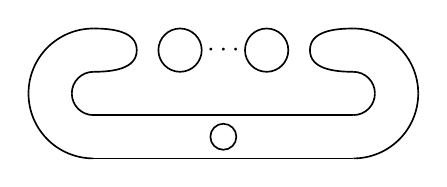
\begin{tikzpicture}[baseline=-0.65ex,scale=0.055]
            \node at (0,10) {$\cdots$};
            \draw[semithick] (-30,  -5) -- (30, -5);
            \draw[semithick] (-30, -15) -- (30,-15);

            \draw[semithick] (0,-10) circle (3);

                % zewnętrzne obręcze -- lewa strona
            \draw[semithick] (-30, 15) to [out=left, in=up]   (-45, 0);
            \draw[semithick] (-30,-15) to [out=left, in=down] (-45, 0);
            \draw[semithick] (-30,  5) to [out=left, in=up]   (-35, 0);
            \draw[semithick] (-30, -5) to [out=left, in=down] (-35, 0);

                % zewnętrzne obręcze -- prawastrona
            \draw[semithick] (30, 15) to [out=right, in=up]   (45,0);
            \draw[semithick] (30,-15) to [out=right, in=down] (45,0);
            \draw[semithick] (30,  5) to [out=right, in=up]   (35,0);
            \draw[semithick] (30, -5) to [out=right, in=down] (35,0);

            \draw[semithick] (-30, 15) to [out=right, in=up] (-20,10);
            \draw[semithick] (-30,  5) to [out=right, in=down] (-20,10);

            \draw[semithick] (30, 15) to [out=left, in=up] (20,10);
            \draw[semithick] (30,  5) to [out=left, in=down] (20,10);

            \draw[semithick] (-10, 10) circle (5);
            \draw[semithick] (10,  10) circle (5);
        \end{tikzpicture}
    \]
\end{comment}
    Wynika stąd, że genus wynosi $\frac 12 (1 - (1+2n) + (2+2n)) = 1$, ponieważ wyznacznik ma wartość $4n+1$,
    węzły $(2n+2)_1$ nie są trywialne i~są parami różne.
\end{proof}

\index{genus|)}

% Koniec podsekcji Genus
